\documentclass[10pt]{article}
\usepackage[margin=0.72in]{geometry}
\usepackage{booktabs,longtable,graphicx,amsmath,xcolor,hyperref,fvextra}
\hypersetup{colorlinks=true,linkcolor=blue,urlcolor=blue}
\newcommand{\NA}{\textemdash}
\begin{document}
\begin{center}
{\Large Heat-flux affinity sweep and Gaussian crossover}\par
\vspace{0.3em}
{\small Frozen $n=10$ Cartesian experiment with equilibrium amendment, 2026-09-04}
\end{center}

\section*{Scope and frozen estimator}
The transported heat in a window is
\[
Q=\frac{Q_L-Q_R}{2},\qquad
\Delta\beta=\frac{1}{T_R}-\frac{1}{T_L}.
\]
Non-overlapping windows are formed within each of 128 independent streams.
The directly sampled fluctuation-relation slope is obtained from raw matched
bins of $\log[p(Q)/p(-Q)]$ against $Q$.  The fixed rule is
$\Delta Q=\operatorname{std}(Q)/20$, at least 10 raw observations on each
side of every accepted bin pair, and the largest contiguous reliable block
that straddles zero.  No plus-four points or extrapolated densities enter the
fit.  Stream bootstrap intervals resample the 128 complete streams.

The Gaussian bulk diagnostics are
\[
a_{\rm Gauss}=\frac{2\langle Q\rangle}{\operatorname{Var}(Q)},\qquad
G_{\rm FT}=\frac{\operatorname{Var}(Q)}{2\langle Q\rangle/\Delta\beta}.
\]
They characterize the CLT crossover but are not substitutes for a directly
sampled negative tail.

\section*{Provenance}
Experiment repository commit: \nolinkurl{e170205c5d9a3d9b2bfca3714a4447fa965a1e40}.\\
Production source commit: \nolinkurl{1905cf4e606a4a7f4dd8930caa64bd4cc861e9d4}.\\
Frozen source SHA-256: \nolinkurl{98e7f8f5f915c8ce02bd8aa10722025c09fd739184b981961692869c9356c0d3}.\\
Driven binary SHA-256: \nolinkurl{4c4880d721733897d200f2601690da873f5b226aaa1013df23df2351c1dfe7d1}.\\
Equilibrium binary SHA-256: \nolinkurl{5fdcd596f0b4da39357a7217fb8b475f14e7b381da08a1208351fccbc008080e}.\\

The four driven runs and the equilibrium amendment use $n=10$, $\gamma=0.1$, $dt=5\times10^{-4}$, burn-in 500, base block duration 20, 8 SIMD batches, 16 lanes, 7,813 blocks per stream, and 1,000,064 blocks per case.
\paragraph{Exact production commands.}
\begin{Verbatim}[fontsize=\scriptsize,breaklines=true,breakanywhere=true]
dbeta_0p027972  /Users/jayleenjiang/NLS_affinity_runtime/experiments/entropy_ft_affinity_sweep_2026-09-03/bin/entropy_ft_affinity sample 6.5 5.5 10 8 500 20 7813 0.0005 2026090401 2 /Users/jayleenjiang/NLS_affinity_runtime/experiments/entropy_ft_affinity_sweep_2026-09-03/raw/dbeta_0p027972_n10 5
dbeta_0p057143  /Users/jayleenjiang/NLS_affinity_runtime/experiments/entropy_ft_affinity_sweep_2026-09-03/bin/entropy_ft_affinity sample 7 5 10 8 500 20 7813 0.0005 2026090402 2 /Users/jayleenjiang/NLS_affinity_runtime/experiments/entropy_ft_affinity_sweep_2026-09-03/raw/dbeta_0p057143_n10 5
dbeta_0p125000  /Users/jayleenjiang/NLS_affinity_runtime/experiments/entropy_ft_affinity_sweep_2026-09-03/bin/entropy_ft_affinity sample 8 4 10 8 500 20 7813 0.0005 2026090403 2 /Users/jayleenjiang/NLS_affinity_runtime/experiments/entropy_ft_affinity_sweep_2026-09-03/raw/dbeta_0p125000_n10 5
dbeta_0p222222  /Users/jayleenjiang/NLS_affinity_runtime/experiments/entropy_ft_affinity_sweep_2026-09-03/bin/entropy_ft_affinity sample 9 3 10 8 500 20 7813 0.0005 2026090404 2 /Users/jayleenjiang/NLS_affinity_runtime/experiments/entropy_ft_affinity_sweep_2026-09-03/raw/dbeta_0p222222_n10 5
dbeta_0p000000  /Users/jayleenjiang/NLS_affinity_runtime/experiments/entropy_ft_affinity_sweep_2026-09-03/bin/entropy_ft_affinity_equilibrium sample 6 6 10 8 500 20 7813 0.0005 2026090405 2 /Users/jayleenjiang/NLS_affinity_runtime/experiments/entropy_ft_affinity_sweep_2026-09-03/raw/dbeta_0p000000_n10 5
\end{Verbatim}
\paragraph{Input hashes.}
\begin{longtable}{lrp{0.62\textwidth}}
\toprule Case & rows & SHA-256 \\
\midrule\endhead
\texttt{dbeta\_0p027972} & 1000064 & \scriptsize\nolinkurl{8b44be37ea8f566fb3862b6cd796dcfcf433be0888752babb876754c84d4c421} \\
\texttt{dbeta\_0p057143} & 1000064 & \scriptsize\nolinkurl{382496fcd194154b0f6d486f2d4da9de80d2d0791f94cb0f3e695d8e666a29cc} \\
\texttt{dbeta\_0p125000} & 1000064 & \scriptsize\nolinkurl{0404492717ce335c1e2eff7970d5d514435fabec9b91604fa92b7d4846cdf685} \\
\texttt{dbeta\_0p222222} & 1000064 & \scriptsize\nolinkurl{342f3783b40db98263cd685c8ab4e531c9d83842db6762b0bd0a06061642958d} \\
\texttt{dbeta\_0p400000} & 1000064 & \scriptsize\nolinkurl{a23806e82f5514a9c3375d10a6644946b6b57d0efe8452b3bbf397b6230f9929} \\
\texttt{dbeta\_0p000000} & 1000064 & \scriptsize\nolinkurl{7fd6827f12b42844de1142613af124702ca5535ba63f3c54ab71006b256aef4d} \\
\bottomrule\end{longtable}
\noindent Full absolute input paths are retained in \texttt{analysis/input\_hashes.csv}.
\section*{Outcome under the frozen gates}
The full-sample $1/t$ intercepts give $a_\infty/\Delta\beta=1.0175,\ 1.0153,\ 1.0220$ at $\Delta\beta=0.027972,\ 0.057143,\ 0.125$, respectively.  These point estimates lie close to the FT reference, but none of the cases reaches the predeclared threshold of 800 valid joint stream-bootstrap intercepts.  Consequently every nonzero-affinity FT verdict is \texttt{UNRESOLVED}; the point estimates alone are not promoted to a pass.
For the equilibrium control, the full-sample intercept is $7.80\times10^{-5}$.  Its $t=20$ direct slope is $1.63\times10^{-4}$ with stream-bootstrap 95\% interval $[-8.98\times10^{-5},\,4.18\times10^{-4}]$, which contains zero.  The joint long-time interval again fails the 800-replicate gate, so the formal equilibrium extrapolation remains \texttt{UNRESOLVED}.
The Gaussian bulk approaches the FT value only at weak drive: $a_{\rm Gauss}/\Delta\beta=0.960,\ 0.931,\ 0.745,\ 0.515,\ 0.301$ as the affinity increases.  At $t=160$, the negative counts fall from 20,136 and 2,997 in the two weakest driven cases to 2, 0, and 0 in the three stronger cases.  This directly records the loss of two-tail support rather than replacing it by a Gaussian estimate.
\section*{Raw window statistics and two-tail fits}
\subsection*{dbeta\_0p027972: $(T_L,T_R)=(6.5,5.5)$, $\Delta\beta=0.027972$}
\scriptsize\begin{longtable}{rrrrrrrrrrr}
\toprule $t$ & $N$ & mean & std & skew & ex.kurt & $n_-$ & $a_{fit}$ & boot.95\% CI & $R^2$ & $a_G$ / $G_{FT}$ \\
\midrule\endhead
20 & 1000064 & 8.9368 & 25.8599 & 0.1348 & 0.3798 & 366513 & 0.02720 & [--,--] & 0.9978 & 0.02673 / 1.0466 \\
40 & 499968 & 17.8742 & 36.3277 & 0.1019 & 0.2084 & 155995 & 0.02758 & [--,--] & 0.9979 & 0.02709 / 1.0326 \\
80 & 249984 & 35.7483 & 51.2908 & 0.0770 & 0.0995 & 60756 & 0.02781 & [0.02736,0.02818] & 0.9979 & 0.02718 / 1.0292 \\
160 & 124928 & 71.4974 & 72.6266 & 0.0512 & 0.0388 & 20136 & 0.02706 & [0.02645,0.02754] & 0.9951 & 0.02711 / 1.0318 \\
320 & 62464 & 142.9947 & 102.6171 & 0.0433 & 0.0109 & 5109 & 0.02778 & [--,--] & 0.9944 & 0.02716 / 1.0299 \\
640 & 31232 & 285.9894 & 145.9539 & 0.0505 & 0.0103 & 764 & 0.03036 & [--,--] & 0.9704 & 0.02685 / 1.0418 \\
\bottomrule\end{longtable}\normalsize
\subsection*{dbeta\_0p057143: $(T_L,T_R)=(7.0,5.0)$, $\Delta\beta=0.057143$}
\scriptsize\begin{longtable}{rrrrrrrrrrr}
\toprule $t$ & $N$ & mean & std & skew & ex.kurt & $n_-$ & $a_{fit}$ & boot.95\% CI & $R^2$ & $a_G$ / $G_{FT}$ \\
\midrule\endhead
20 & 1000064 & 17.7373 & 26.2279 & 0.2518 & 0.4064 & 248420 & 0.05487 & [0.05446,0.05523] & 0.9993 & 0.05157 / 1.1081 \\
40 & 499968 & 35.4752 & 36.8119 & 0.1869 & 0.2167 & 82050 & 0.05602 & [--,--] & 0.9991 & 0.05236 / 1.0914 \\
80 & 249984 & 70.9503 & 51.9375 & 0.1401 & 0.0936 & 20447 & 0.05651 & [--,--] & 0.9986 & 0.05260 / 1.0863 \\
160 & 124928 & 141.8966 & 73.3519 & 0.0951 & 0.0409 & 2997 & 0.05614 & [--,--] & 0.9928 & 0.05274 / 1.0834 \\
320 & 62464 & 283.7931 & 103.2913 & 0.0737 & 0.0348 & 150 & 0.05978 & [--,--] & 0.6020 & 0.05320 / 1.0741 \\
640 & 31232 & 567.5862 & 145.5179 & 0.0377 & 0.0130 & 1 & \textsc{unres.} & -- & -- & 0.05361 / 1.0659 \\
\bottomrule\end{longtable}\normalsize
\subsection*{dbeta\_0p125000: $(T_L,T_R)=(8.0,4.0)$, $\Delta\beta=0.125000$}
\scriptsize\begin{longtable}{rrrrrrrrrrr}
\toprule $t$ & $N$ & mean & std & skew & ex.kurt & $n_-$ & $a_{fit}$ & boot.95\% CI & $R^2$ & $a_G$ / $G_{FT}$ \\
\midrule\endhead
20 & 1000064 & 34.8992 & 27.7171 & 0.4529 & 0.5303 & 88761 & 0.11337 & [--,--] & 0.9995 & 0.09086 / 1.3758 \\
40 & 499968 & 69.7973 & 38.8933 & 0.3447 & 0.2789 & 12744 & 0.11966 & [--,--] & 0.9975 & 0.09228 / 1.3545 \\
80 & 249984 & 139.5947 & 54.7524 & 0.2520 & 0.1553 & 661 & 0.12460 & [--,--] & 0.9866 & 0.09313 / 1.3422 \\
160 & 124928 & 279.1903 & 77.2501 & 0.1806 & 0.0808 & 2 & \textsc{unres.} & -- & -- & 0.09357 / 1.3359 \\
320 & 62464 & 558.3805 & 109.0295 & 0.1323 & 0.0777 & 0 & \textsc{unres.} & -- & -- & 0.09394 / 1.3306 \\
640 & 31232 & 1116.7611 & 153.4323 & 0.1020 & 0.0404 & 0 & \textsc{unres.} & -- & -- & 0.09488 / 1.3175 \\
\bottomrule\end{longtable}\normalsize
\subsection*{dbeta\_0p222222: $(T_L,T_R)=(9.0,3.0)$, $\Delta\beta=0.222222$}
\scriptsize\begin{longtable}{rrrrrrrrrrr}
\toprule $t$ & $N$ & mean & std & skew & ex.kurt & $n_-$ & $a_{fit}$ & boot.95\% CI & $R^2$ & $a_G$ / $G_{FT}$ \\
\midrule\endhead
20 & 1000064 & 50.8282 & 29.9660 & 0.5614 & 0.5940 & 24798 & 0.17618 & [0.17407,0.17782] & 0.9994 & 0.11321 / 1.9630 \\
40 & 499968 & 101.6576 & 42.1593 & 0.4311 & 0.3267 & 985 & 0.19148 & [--,--] & 0.9901 & 0.11439 / 1.9427 \\
80 & 249984 & 203.3151 & 59.3516 & 0.3233 & 0.1607 & 3 & \textsc{unres.} & -- & -- & 0.11543 / 1.9251 \\
160 & 124928 & 406.6254 & 83.9248 & 0.2323 & 0.0889 & 0 & \textsc{unres.} & -- & -- & 0.11546 / 1.9246 \\
320 & 62464 & 813.2508 & 119.0787 & 0.1714 & 0.0688 & 0 & \textsc{unres.} & -- & -- & 0.11471 / 1.9373 \\
640 & 31232 & 1626.5015 & 168.5450 & 0.0984 & 0.0109 & 0 & \textsc{unres.} & -- & -- & 0.11451 / 1.9406 \\
\bottomrule\end{longtable}\normalsize
\subsection*{dbeta\_0p400000: $(T_L,T_R)=(10.0,2.0)$, $\Delta\beta=0.400000$}
\scriptsize\begin{longtable}{rrrrrrrrrrr}
\toprule $t$ & $N$ & mean & std & skew & ex.kurt & $n_-$ & $a_{fit}$ & boot.95\% CI & $R^2$ & $a_G$ / $G_{FT}$ \\
\midrule\endhead
20 & 1000064 & 64.2424 & 32.6857 & 0.6006 & 0.6213 & 7941 & 0.21573 & [--,--] & 0.9985 & 0.12026 / 3.3260 \\
40 & 499968 & 128.4849 & 45.9342 & 0.4603 & 0.3523 & 80 & \textsc{unres.} & -- & -- & 0.12179 / 3.2844 \\
80 & 249984 & 256.9699 & 64.7162 & 0.3377 & 0.1853 & 0 & \textsc{unres.} & -- & -- & 0.12271 / 3.2597 \\
160 & 124928 & 513.9476 & 91.2279 & 0.2361 & 0.0836 & 0 & \textsc{unres.} & -- & -- & 0.12351 / 3.2387 \\
320 & 62464 & 1027.8951 & 128.6532 & 0.1634 & 0.0240 & 0 & \textsc{unres.} & -- & -- & 0.12420 / 3.2205 \\
640 & 31232 & 2055.7903 & 182.2058 & 0.1061 & 0.0165 & 0 & \textsc{unres.} & -- & -- & 0.12385 / 3.2298 \\
\bottomrule\end{longtable}\normalsize
\subsection*{dbeta\_0p000000: $(T_L,T_R)=(6.0,6.0)$, $\Delta\beta=0$}
\scriptsize\begin{longtable}{rrrrrrrrrrr}
\toprule $t$ & $N$ & mean & std & skew & ex.kurt & $n_-$ & $a_{fit}$ & boot.95\% CI & $R^2$ & $a_G$ / $G_{FT}$ \\
\midrule\endhead
20 & 1000064 & 0.0306 & 25.7283 & -0.0027 & 0.3783 & 499786 & 1.63012e-04 & [-8.97958e-05,4.18259e-04] & 0.0214 & 9.24910e-05 / -- \\
40 & 499968 & 0.0610 & 36.1107 & -0.0068 & 0.2064 & 249282 & -1.10678e-05 & [--,--] & 1.0247e-04 & 9.34879e-05 / -- \\
80 & 249984 & 0.1219 & 50.8838 & -0.0029 & 0.1190 & 124666 & 3.89544e-05 & [--,--] & 0.0010 & 9.41668e-05 / -- \\
160 & 124928 & 0.2379 & 71.8208 & -3.2658e-04 & 0.0612 & 62425 & 2.26664e-04 & [--,--] & 0.0551 & 9.22287e-05 / -- \\
320 & 62464 & 0.4757 & 101.3193 & -0.0103 & 0.0283 & 31032 & -2.82407e-06 & [--,--] & 6.7076e-06 & 9.26856e-05 / -- \\
640 & 31232 & 0.9515 & 143.2340 & 0.0089 & -0.0130 & 15544 & 1.20689e-04 & [--,--] & 0.0124 & 9.27544e-05 / -- \\
\bottomrule\end{longtable}\normalsize
\section*{Long-time extrapolation}
\begin{longtable}{lrrrrrrl}
\toprule Case & $\Delta\beta$ & resolved $t$ & $a_\infty$ & 95\% CI & $a_\infty/\Delta\beta$ & ratio CI & status \\
\midrule\endhead
\texttt{dbeta\_0p027972} & 0.027972 & 20;40;80;160;320;640 & 0.02846 & [--,--] & -- & [--,--] & UNRESOLVED \\
\texttt{dbeta\_0p057143} & 0.057143 & 20;40;80;160;320 & 0.05802 & [--,--] & -- & [--,--] & UNRESOLVED \\
\texttt{dbeta\_0p125000} & 0.125000 & 20;40;80 & 0.12775 & [--,--] & -- & [--,--] & UNRESOLVED \\
\texttt{dbeta\_0p222222} & 0.222222 & 20;40 & -- & [--,--] & -- & [--,--] & UNRESOLVED \\
\texttt{dbeta\_0p400000} & 0.400000 & 20 & -- & [--,--] & -- & [--,--] & UNRESOLVED \\
\texttt{dbeta\_0p000000} & 0 & 20;40;80;160;320;640 & 7.80343e-05 & [--,--] & -- & [--,--] & UNRESOLVED \\
\bottomrule\end{longtable}
\section*{Crossover summary}
\scriptsize\begin{longtable}{rrrrrrrrl}
\toprule $\Delta\beta$ & $a_\infty/\Delta\beta$ & ratio CI & $a_G/\Delta\beta$ & $G_{FT}(640)$ & skew(160) & ex.kurt(160) & $n_-(160)$ & status \\
\midrule\endhead
0 & -- & [--,--] & -- & -- & -3.2658e-04 & 0.0612 & 62425 & UNRESOLVED \\
0.027972 & -- & [--,--] & 0.9599 & 1.0418 & 0.0512 & 0.0388 & 20136 & UNRESOLVED \\
0.057143 & -- & [--,--] & 0.9310 & 1.0659 & 0.0951 & 0.0409 & 2997 & UNRESOLVED \\
0.125000 & -- & [--,--] & 0.7450 & 1.3175 & 0.1806 & 0.0808 & 2 & UNRESOLVED \\
0.222222 & -- & [--,--] & 0.5147 & 1.9406 & 0.2323 & 0.0889 & 0 & UNRESOLVED \\
0.400000 & -- & [--,--] & 0.3007 & 3.2298 & 0.2361 & 0.0836 & 0 & UNRESOLVED \\
\bottomrule\end{longtable}\normalsize
\section*{Figures}
\begin{figure}[ht]
\centering
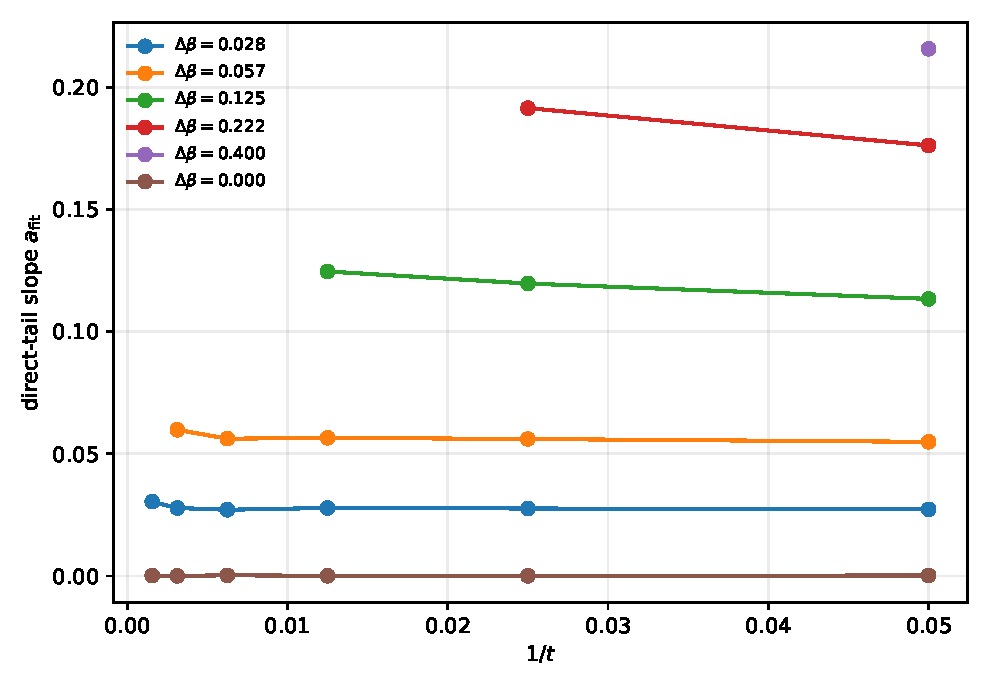
\includegraphics[width=0.76\textwidth]{../figures/a_fit_vs_inverse_time.pdf}
\caption{Direct matched-bin slopes against inverse window duration.}
\end{figure}
\begin{figure}[ht]
\centering
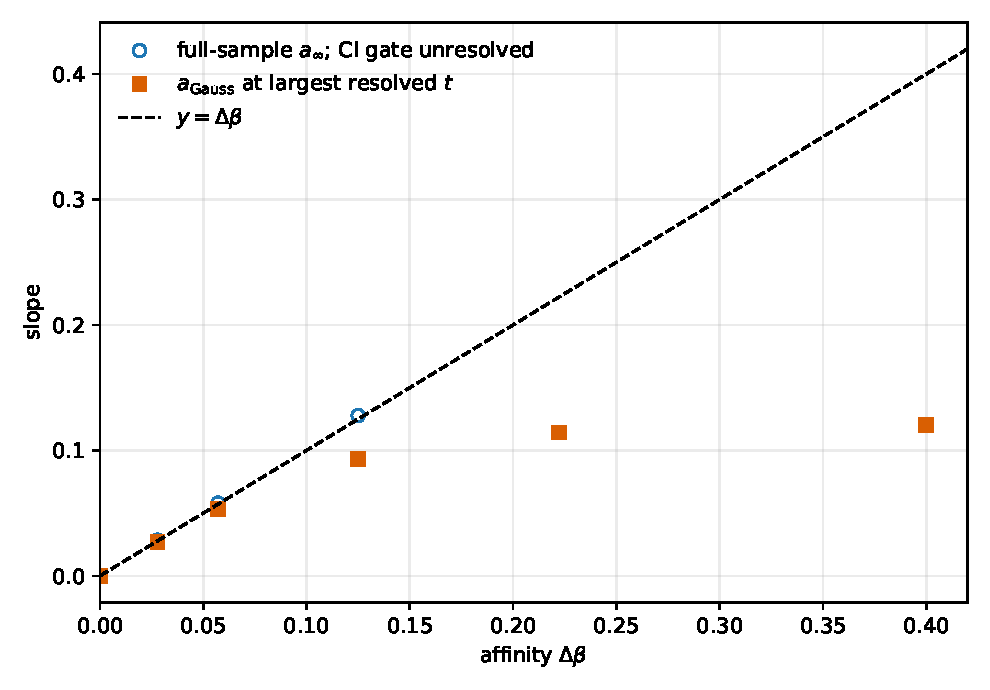
\includegraphics[width=0.76\textwidth]{../figures/slope_crossover_vs_affinity.pdf}
\caption{Extrapolated direct-tail slopes and Gaussian bulk slopes against affinity.}
\end{figure}
\begin{figure}[ht]
\centering

\includegraphics[width=0.76\textwidth]{../figures/gaussFT_vs_affinity.pdf}
\caption{Gaussian FT ratio at $t=640$ across affinity.}
\end{figure}

\section*{Equilibrium row and claim boundary}
The added $(6,6)$ production uses the same $n=10$ dynamics, integration step,
burn-in, stream count, and block count as the driven cases.  At
$\Delta\beta=0$, ratios that divide by $\Delta\beta$ and $G_{\rm FT}$ are
undefined and are reported as dashes.  The direct asymmetry-slope reference is
zero; its extrapolated confidence interval is tested against zero rather than
against a ratio of one.

The complete raw positive/negative counts used by every fit are in
\texttt{analysis/symmetric\_bin\_raw\_counts.csv}; all per-window statistics
are in \texttt{analysis/window\_summary.csv}.  A case labelled
\texttt{CONSISTENT\_WITH\_FT} means only that the predeclared extrapolated
confidence interval includes the reference.  It is not a proof.  A case whose
interval excludes the reference is labelled \texttt{FAIL}; insufficient raw
two-tail support remains \texttt{UNRESOLVED}.  The label
\texttt{CONSISTENT\_WITH\_EQUILIBRIUM} has the corresponding limited meaning
for the zero-affinity control.
\end{document}
